\chapter{Compras}
\label{mod:10-compras}

\section{Propósito}
\label{sec:compras-proposito}

Gestiona el ciclo de abastecimiento de mercadería desde proveedores externos: alta de proveedores, órdenes de compra (OC), registro de la factura del proveedor, recepción física de la mercadería (con generación de lotes y stock) y devoluciones al proveedor.

\section{Entidades principales}
\label{sec:compras-entidades}

\begin{longtable}{p{3.6cm}p{9.6cm}}
\caption{Entidades principales del módulo de Compras.}
\label{tab:compras-entidades}\\
\toprule
\textbf{Entidad} & \textbf{Rol} \\
\midrule
\endfirsthead
\toprule
\textbf{Entidad} & \textbf{Rol} \\
\midrule
\endhead
\bottomrule
\endfoot
\code{Proveedor} / \code{ProveedorContacto} & Catálogo de proveedores (compartido con Laboratorio vía el flag \code{EsLaboratorio}). \\
\code{PedidoProveedor} / \code{Pedido}\allowbreak \code{Proveedor}\allowbreak \code{Item} & La orden de compra (OC) y sus líneas. \\
\code{FacturaCompra} (subtipo de \code{Egreso}, TPH) & Factura del proveedor --- ver Capítulo~\ref{mod:11-caja-y-egresos} (Caja y Egresos) para la jerarquía completa. \\
\code{Recepcion}\allowbreak \code{Mercaderia} / \code{Recepcion}\allowbreak \code{Mercaderia}\allowbreak \code{Item} & Recepción física (puede ser parcial, una OC admite varias). \\
\code{StockLote} & Generado por cada línea de recepción con lote/vencimiento (ver Capítulo~\ref{mod:07-inventario-catalogo}). \\
\code{Devolucion}\allowbreak \code{Proveedor} & Devolución de mercadería ya recibida hacia el proveedor. \textbf{No confundir con} \code{Devolucion}/\code{DevolucionLinea}, que es la devolución/cambio del lado del cliente en una \code{Venta} (Capítulo~\ref{mod:08-ventas}) --- son dos entidades distintas sin relación entre sí, solo comparten la palabra ``devolución''. \\
\end{longtable}

Ver el capítulo de Modelo de Datos (\S\ref{sec:modelo-datos}, Grupo C) para el diccionario de datos completo.

\section{Reglas de negocio clave}
\label{sec:compras-reglas}

\begin{itemize}
  \item Una OC solo se puede \textbf{editar} (reemplazo completo de ítems) mientras está en \code{Borrador}.
  \item Una OC \textbf{no se puede cancelar} si ya está \code{RecibidaTotal}.
  \item Las \textbf{devoluciones a proveedor} (\code{Devolucion}\allowbreak \code{Proveedor}) solo se permiten sobre OCs con mercadería recibida (\code{RecibidaTotal}/\code{RecibidaParcial}), y la cantidad a devolver no puede superar la cantidad recibida del ítem. Cada devolución genera un \code{MovimientoStock} de \code{Salida} en estado \code{Aprobado} (descuenta stock inmediatamente, sin flujo de aprobación adicional).
  \item Alta de proveedor exige \textbf{al menos un contacto con nombre} (validado en backend y frontend).
  \item El pago en efectivo de una factura de compra exige una \code{SesionCaja} \textbf{abierta} en la sucursal --- si no hay, la operación falla explícitamente en vez de crear un movimiento huérfano.
  \item \textbf{El ciclo de una OC es \code{Borrador} $\to$ \code{Confirmada} $\to$ \code{Facturada} $\to$ \code{RecibidaParcial}/\allowbreak \code{RecibidaTotal}.} La factura del proveedor se registra apenas la OC está \code{Confirmada} (\code{Registrar}\allowbreak \code{Factura}\allowbreak \code{Async}), antes de la recepción física de la mercadería; recién con la factura registrada (\code{Facturada} o \code{RecibidaParcial}) se pueden aceptar recepciones (\code{Recepciones}\allowbreak \code{Service}).
\end{itemize}

\section{Endpoints}
\label{sec:compras-endpoints}

Ver el Apéndice de Referencia de API § Compras para la tabla completa (\code{ComprasController}, \code{Proveedores}\allowbreak \code{Controller}, \code{Facturas}\allowbreak \code{Compra}\allowbreak \code{Controller}, \code{Recepciones}\allowbreak \code{Controller}).

\begin{longtable}{p{1.3cm}p{5.6cm}p{6.3cm}}
\caption{Endpoints de transición de estado de la OC.}
\label{tab:compras-endpoints}\\
\toprule
\textbf{Método} & \textbf{Ruta} & \textbf{Transición / acción} \\
\midrule
\endfirsthead
\toprule
\textbf{Método} & \textbf{Ruta} & \textbf{Transición / acción} \\
\midrule
\endhead
\bottomrule
\endfoot
POST & \code{/}\allowbreak \code{api/}\allowbreak \code{compras/}\allowbreak \code{pedidos} & Crea OC en \code{Borrador} \\
PUT & \code{/}\allowbreak \code{api/}\allowbreak \code{compras/}\allowbreak \code{pedidos/}\allowbreak \code{{id}/confirmar} & \code{Borrador} $\to$ \code{Confirmada} (policy \code{aprobar_pedidos}, distinta de crear/editar) \\
POST & \code{/}\allowbreak \code{api/}\allowbreak \code{compras/}\allowbreak \code{pedidos/}\allowbreak \code{{id}/factura} & \code{Confirmada} $\to$ \code{Facturada} \\
POST & \code{/}\allowbreak \code{api/}\allowbreak \code{compras/}\allowbreak \code{recepciones} & \code{Facturada}/\code{RecibidaParcial} $\to$ \code{RecibidaParcial}/\code{RecibidaTotal} (según ítems pendientes) \\
POST & \code{/}\allowbreak \code{api/}\allowbreak \code{compras/}\allowbreak \code{pedidos/}\allowbreak \code{{id}/devolucion} & Devolución sobre OC recibida (no cambia el estado de la OC) \\
PUT & \code{/}\allowbreak \code{api/}\allowbreak \code{compras/}\allowbreak \code{pedidos/}\allowbreak \code{{id}/cancelar} & $\to$ \code{Cancelada} (policy OR: creador \code{gestionar_pedidos} o aprobador \code{aprobar_pedidos}) \\
\end{longtable}

\section{Flujo típico}
\label{sec:compras-flujo}

El ciclo se muestra en dos figuras: desde la creación de la OC hasta la factura del proveedor (Figura~\ref{fig:seq-compras-oc-factura}), y desde la recepción física hasta una eventual devolución (Figura~\ref{fig:seq-compras-recepcion}).

\begin{figure}[htbp]
\centering
\begin{tikzpicture}[node distance=3.2cm]
  \node[actor] (u) {Usuario};
  \node[actor, right=of u] (oc) {PedidoProveedor};
  \node[actor, right=of oc] (f) {FacturaCompra};

  \draw[lineavida] (u.south) -- ++(0,-5.6);
  \draw[lineavida] (oc.south) -- ++(0,-5.6);
  \draw[lineavida] (f.south) -- ++(0,-5.6);

  \draw[mensaje] ($(u.south)+(0,-0.9)$) -- node[above,font=\scriptsize]{CrearPedidoAsync} node[below,font=\tiny\itshape]{Estado = Borrador} ($(oc.south)+(0,-0.9)$);
  \draw[mensaje] ($(u.south)+(0,-2.3)$) -- node[above,font=\scriptsize]{EditarPedidoAsync} node[below,font=\tiny\itshape]{solo mientras Borrador} ($(oc.south)+(0,-2.3)$);
  \draw[mensaje] ($(u.south)+(0,-3.7)$) -- node[above,font=\scriptsize]{ConfirmarPedidoAsync (aprobar\_pedidos)} node[below,font=\tiny\itshape]{Estado = Confirmada} ($(oc.south)+(0,-3.7)$);
  \draw[mensaje] ($(u.south)+(0,-5.1)$) -- node[above,font=\scriptsize,align=center]{RegistrarFacturaAsync\\(efectivo exige SesionCaja abierta)} node[below,font=\tiny\itshape]{Estado OC = Facturada} ($(f.south)+(0,-5.1)$);
\end{tikzpicture}
\caption{Desde la creación de la orden de compra hasta el registro de la factura del proveedor. La factura se registra \textbf{antes} de la recepción física.}
\label{fig:seq-compras-oc-factura}
\end{figure}

\begin{figure}[htbp]
\centering
% node distance corto y nombres en dos lineas: con 3.2cm la figura mide
% ~18cm y no entra en los 16cm de ancho de texto.
\begin{tikzpicture}[node distance=2.2cm]
  \node[actor] (u) {Usuario};
  \node[actor, right=of u] (r) {Recepcion\\Mercaderia};
  \node[actor, right=of r] (s) {StockLote /\\MovimientoStock};

  \draw[lineavida] (u.south) -- ++(0,-5.6);
  \draw[lineavida] (r.south) -- ++(0,-5.6);
  \draw[lineavida] (s.south) -- ++(0,-5.6);

  \draw[mensaje] ($(u.south)+(0,-0.9)$) -- node[above,font=\scriptsize]{RegistrarRecepcionAsync (1 o más veces)} ($(r.south)+(0,-0.9)$);
  \draw[mensaje] ($(r.south)+(0,-2.3)$) -- node[above,font=\scriptsize,align=center]{genera StockLote +\\MovimientoStock Entrada/Aprobado por ítem} ($(s.south)+(0,-2.3)$);
  \node[font=\tiny\itshape] at ($(r)+(0,-3.3)$) {Estado OC = RecibidaParcial $\to$ RecibidaTotal (cuando no quedan pendientes)};
  \draw[mensaje] ($(u.south)+(0,-4.5)$) -- node[above,font=\scriptsize]{RegistrarDevolucionAsync (opt.\ sobre OC recibida)} ($(r.south)+(0,-4.5)$);
  \draw[mensaje] ($(r.south)+(0,-5.5)$) -- node[above,font=\scriptsize]{MovimientoStock Salida/Aprobado} ($(s.south)+(0,-5.5)$);
\end{tikzpicture}
\caption{Recepción física (una o más, parcial) y devolución opcional al proveedor.}
\label{fig:seq-compras-recepcion}
\end{figure}

\section{Vistas de frontend}
\label{sec:compras-frontend}

Rutas bajo \code{/compras/*} (\code{SIGA-Web/}\allowbreak \code{src/}\allowbreak \code{router/}\allowbreak \code{index.}\allowbreak \code{ts}):

\begin{longtable}{p{8cm}p{6cm}}
\caption{Vistas de frontend del módulo Compras.}
\label{tab:compras-vistas}\\
\toprule
\textbf{Vista} & \textbf{Ruta} \\
\midrule
\endfirsthead
\toprule
\textbf{Vista} & \textbf{Ruta} \\
\midrule
\endhead
\bottomrule
\endfoot
\code{PedidosView.vue} & \code{/compras/oc} \\
\code{OcFormView.vue} & \code{/compras/oc/nueva}, \code{/}\allowbreak \code{compras/}\allowbreak \code{oc/}\allowbreak \code{:id/}\allowbreak \code{editar} \\
\code{OcDetailView.vue} & \code{/compras/oc/:id} \\
\code{OcAprobacionView.}\allowbreak \code{vue} & \code{/}\allowbreak \code{compras/}\allowbreak \code{aprobaciones} \\
\code{FacturasCompraView.}\allowbreak \code{vue} / \code{FacturaFormView.}\allowbreak \code{vue} / \code{FacturaDetailView.}\allowbreak \code{vue} & \code{/}\allowbreak \code{compras/}\allowbreak \code{facturas*} \\
\code{RecepcionesView.}\allowbreak \code{vue} / \code{RecepcionFormView.}\allowbreak \code{vue} / \code{RecepcionDetailView.}\allowbreak \code{vue} & \code{/}\allowbreak \code{compras/}\allowbreak \code{recepciones*} \\
\code{ProveedoresView.}\allowbreak \code{vue} & ruta propia, fuera de \code{/compras} \\
\code{ReportesComprasView.}\allowbreak \code{vue} & \code{/compras/reportes} \\
\end{longtable}

No hay una vista dedicada a \code{Devolucion}\allowbreak \code{Proveedor} --- la acción vive embebida en \code{OcDetailView.vue}.

\section{Interfaz}
\label{sec:compras-interfaz}

\begin{figure}[htbp]
\centering
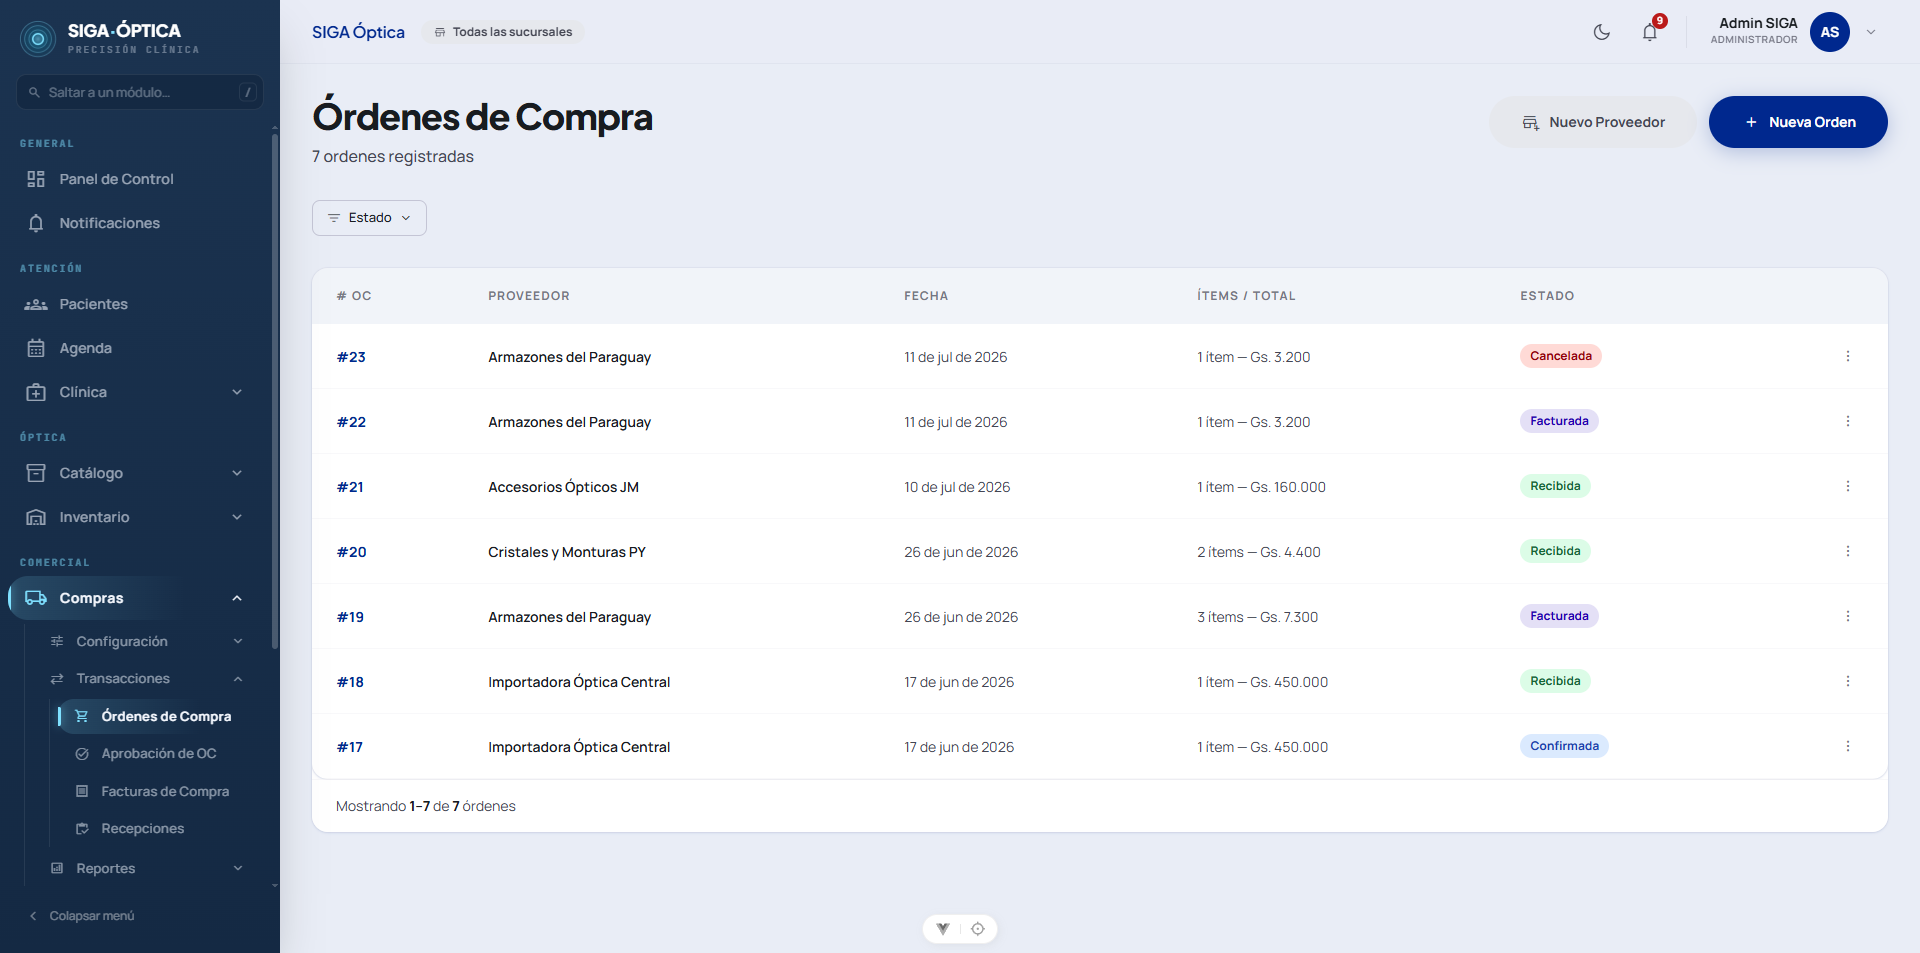
\includegraphics[width=0.95\textwidth]{imagenes/mod10-compras-oc.png}
\caption{Listado de órdenes de compra a proveedores, con la cantidad de ítems, el total y su estado.}
\label{fig:mod10-compras}
\end{figure}

\section{Estado}
\label{sec:compras-estado}

\Implementado\ end-to-end.
